\documentclass[11pt]{article}

% Packages
\usepackage[utf8]{inputenc}
\usepackage[margin=1in]{geometry}
\usepackage{graphicx}
\usepackage{amsmath}
\usepackage{amssymb}
\usepackage{hyperref}
\usepackage{booktabs}
\usepackage{cite}
\usepackage{tikz}
\usepackage{xcolor}
\usepackage{listings}
\usetikzlibrary{shapes.geometric, arrows.meta, positioning, fit, backgrounds, shadows}

% Define colors (Professional grayscale palette)
\definecolor{boxgray}{RGB}{240, 240, 240}
\definecolor{darkgray}{RGB}{100, 100, 100}
\definecolor{medgray}{RGB}{160, 160, 160}
\definecolor{lightgray}{RGB}{220, 220, 220}
\definecolor{codebg}{RGB}{250, 250, 250}

% TikZ styles for architecture diagram (Clean, simple style)
\tikzstyle{layer} = [rectangle, minimum width=5cm, minimum height=1cm, text centered, align=center, draw=black, line width=0.8pt, fill=boxgray, font=\small]
\tikzstyle{component} = [rectangle, minimum width=2.8cm, minimum height=0.9cm, text centered, align=center, draw=darkgray, line width=0.6pt, fill=white, font=\footnotesize]
\tikzstyle{arrow} = [thick,->,>=stealth,line width=0.8pt]
\tikzstyle{data} = [rectangle, draw=medgray, line width=0.6pt, minimum width=3cm, minimum height=0.7cm, text centered, align=center, fill=white, font=\footnotesize]

% Listings style for code (Clean monochrome)
\lstdefinestyle{cleancoding}{
    backgroundcolor=\color{codebg},
    commentstyle=\color{darkgray}\itshape,
    keywordstyle=\bfseries,
    basicstyle=\ttfamily\small,
    breakatwhitespace=false,
    breaklines=true,
    captionpos=b,
    keepspaces=true,
    showspaces=false,
    showstringspaces=false,
    showtabs=false,
    tabsize=2,
    frame=single,
    rulecolor=\color{medgray},
    xleftmargin=2em,
    framexleftmargin=1.5em
}

\lstset{style=cleancoding}

% Title and authors
\title{\textbf{AlphaGenome MCP Server: A Proof-of-Concept Natural Language Interface for AI-Powered Regulatory Genomics Analysis}}

\author{
Taeho Jo\\
\textit{Department of Radiology and Imaging Sciences}\\
\textit{Indiana University School of Medicine}\\
\texttt{tjo@iu.edu}
}

\date{\today}

\begin{document}

\maketitle

\begin{abstract}
The integration of artificial intelligence into genomic analysis workflows remains technically challenging, requiring substantial programming expertise and limiting accessibility for clinical researchers and geneticists. We present AlphaGenome MCP Server, a Model Context Protocol (MCP) implementation that provides natural language access to Google DeepMind's AlphaGenome variant effect prediction API. The server enables researchers to query genetic variants using simple natural language commands, reducing per-query code complexity by approximately 40$\times$ compared to traditional API usage. We implemented 20 specialized analysis tools as lightweight wrappers around a single API endpoint, demonstrating how wrapper architecture reduces implementation complexity while providing diverse analytical capabilities. All tools call the same underlying \texttt{predict\_variant()} API but differ in parameter configuration and output formatting. Validation tests with Alzheimer's disease-associated variants demonstrated successful execution across pathogenicity assessment, tissue-specific analysis, transcription factor binding analysis, chromatin impact assessment, protective vs. risk allele comparison, batch pathogenicity filtering, and comprehensive clinical report generation. The system successfully performed complex multi-variant and multi-tissue analyses, including direct comparison of APOE risk alleles and tissue-specific effect profiling. This work demonstrates how wrapper-based MCP implementations can lower technical barriers to advanced genomics tools while maintaining full access to underlying AI model capabilities. The system is available as open-source software at \url{https://github.com/taehojo/alphagenome-mcp}.
\end{abstract}

\noindent\textbf{Keywords:} natural language interface, genomic variant analysis, Model Context Protocol, AlphaGenome, wrapper architecture, regulatory genomics

\section{Introduction}

The advent of deep learning in genomics has produced powerful predictive models for variant effect prediction, including AlphaGenome~\cite{alphagenome2025}, Enformer~\cite{avsec2021}, and other transformer-based architectures. AlphaGenome, developed by Google DeepMind, represents a state-of-the-art system capable of predicting regulatory impacts across multiple molecular modalities at single base-pair resolution. However, despite their predictive power, these tools remain largely inaccessible to clinical researchers and geneticists who lack extensive programming expertise.

Current genomic analysis workflows present significant technical barriers to adoption. Researchers must first install and configure complex Python environments with specific dependency versions, then write substantial boilerplate code for API authentication and error handling. They must manually parse and format prediction outputs, and finally implement custom visualization and interpretation logic. This multi-step process limits the adoption of AI-powered genomics tools in clinical and translational research settings, where rapid variant interpretation is increasingly critical for precision medicine initiatives.

The Model Context Protocol (MCP), developed by Anthropic, provides a standardized interface for integrating external tools and data sources with large language models. MCP enables natural language interaction with specialized computational tools through a simple client-server architecture. In this architecture, the MCP client (such as Claude Desktop) handles natural language understanding, while the MCP server exposes domain-specific tools via standardized JSON schemas. Communication occurs over stdio, HTTP, or other transports, creating a seamless bridge between conversational AI and computational tools.

This architecture is particularly well-suited for genomics applications, where researchers benefit from conversational interfaces that can translate questions like ``What is the regulatory impact of rs429358?'' into appropriate API calls without requiring programming knowledge. We developed AlphaGenome MCP Server as a proof-of-concept to demonstrate three objectives: enabling natural language queries for AlphaGenome predictions without programming requirements, providing access to multiple AlphaGenome modalities through simple interfaces, and achieving response times suitable for interactive research workflows. This work focuses on demonstrating feasibility and usability rather than comprehensive validation or accuracy benchmarking.

\section{Methods}

\subsection{System Architecture}

AlphaGenome MCP Server implements a multi-tier architecture bridging TypeScript-based MCP protocol handling with Python-based AlphaGenome SDK access (Figure~\ref{fig:architecture}). The system consists of four primary layers. The MCP layer, implemented in TypeScript, handles protocol communication with Claude Desktop via stdio transport. The API client layer manages tool routing, input validation, and output formatting. The Python bridge layer interfaces with the AlphaGenome SDK via subprocess communication, enabling the TypeScript server to access Python-only functionality while maintaining non-blocking asynchronous operation critical for MCP protocol compliance. Finally, the AlphaGenome API layer provides Google DeepMind's prediction service.

\begin{figure}[t]
\centering
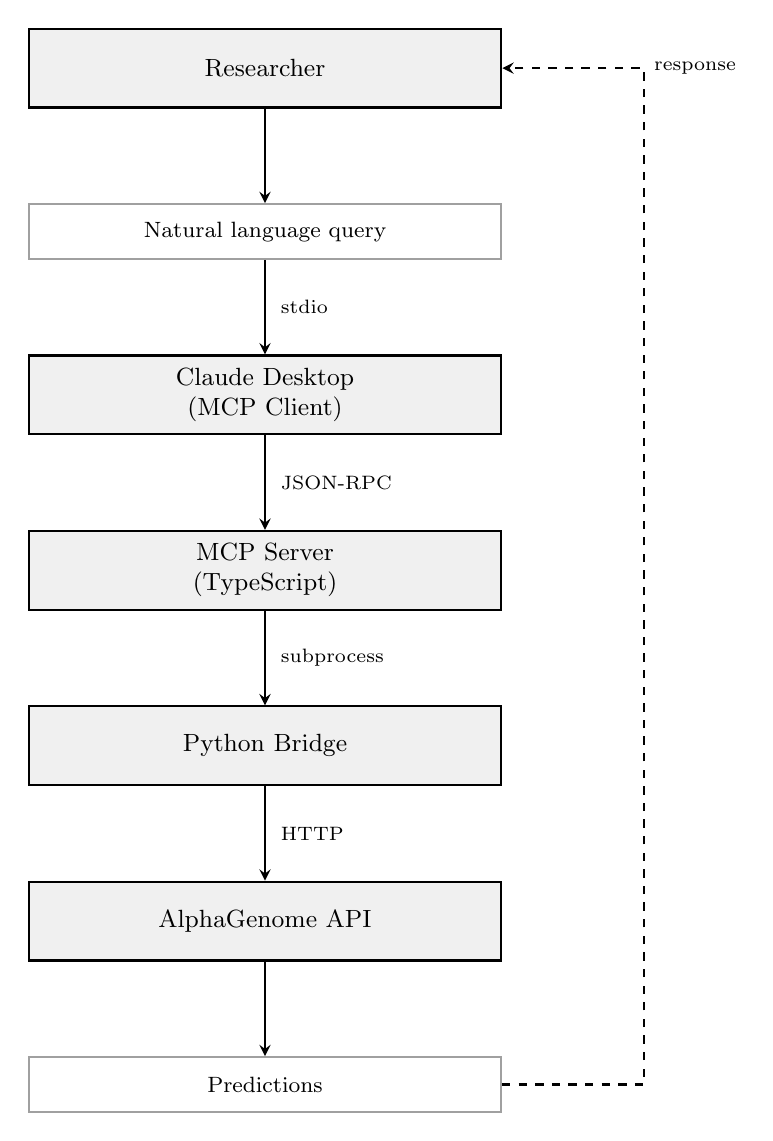
\begin{tikzpicture}[node distance=1.4cm]

% All components with consistent width, vertical flow
\node (researcher) [layer, minimum width=6cm] {Researcher};
\node (query) [data, below=1.2cm of researcher, minimum width=6cm] {Natural language query};
\node (claude) [layer, below=1.2cm of query, minimum width=6cm] {Claude Desktop\\(MCP Client)};
\node (server) [layer, below=1.2cm of claude, minimum width=6cm] {MCP Server\\(TypeScript)};
\node (bridge) [layer, below=1.2cm of server, minimum width=6cm] {Python Bridge};
\node (api) [layer, below=1.2cm of bridge, minimum width=6cm] {AlphaGenome API};
\node (result) [data, below=1.2cm of api, minimum width=6cm] {Predictions};

% Forward arrows (request flow)
\draw [arrow] (researcher) -- (query);
\draw [arrow] (query) -- node[right, font=\scriptsize, xshift=2pt] {stdio} (claude);
\draw [arrow] (claude) -- node[right, font=\scriptsize, xshift=2pt] {JSON-RPC} (server);
\draw [arrow] (server) -- node[right, font=\scriptsize, xshift=2pt] {subprocess} (bridge);
\draw [arrow] (bridge) -- node[right, font=\scriptsize, xshift=2pt] {HTTP} (api);
\draw [arrow] (api) -- (result);

% Return path - go around on the right side
\draw [arrow, dashed] (result.east) -- ++(1.8,0) |- (researcher.east) node[midway, right, font=\scriptsize] {response};

\end{tikzpicture}
\caption{\textbf{System architecture.} The MCP server connects natural language queries to the AlphaGenome API through a four-layer architecture. Solid arrows show request flow; dashed arrow shows response path.}
\label{fig:architecture}
\end{figure}

The server exposes three primary tools via MCP protocol. The \texttt{predict\_variant\_effect} tool analyzes single genetic variants, accepting inputs including chromosome, position, reference allele, alternate allele, optional tissue type, and optional output types. It returns predictions for RNA expression, splicing, transcription factor binding, chromatin accessibility, histone modifications, and 3D chromatin structure at varying resolutions depending on modality. The \texttt{batch\_score\_variants} tool prioritizes multiple variants (up to 100) by regulatory impact using configurable scoring metrics. It outputs ranked variants with impact scores and regulatory effect predictions, enabling batch analysis workflows. The \texttt{analyze\_region} tool identifies regulatory elements in genomic regions between 1 kb and 1 Mb in size, predicting promoters, enhancers, transcription factor binding sites, and chromatin states.

The Python bridge script (\texttt{alphagenome\_bridge.py}) implements JSON-based request/response communication via stdin/stdout. A typical request includes an action identifier, API key, and parameter dictionary specifying the genomic coordinates and analysis options. This architecture enables seamless integration between the TypeScript MCP server and Python-exclusive AlphaGenome SDK while maintaining the asynchronous operation required by the MCP protocol specification.

All tool inputs undergo comprehensive validation using Zod schemas before API submission. Chromosome specifications are pattern-matched for chr1-22, chrX, and chrY formats. Positions are validated as positive integers with appropriate range checking. Alleles are validated against A/T/G/C nucleotides with length constraints, and tissue types are validated against UBERON ontology terms. Invalid inputs return structured error messages via MCP protocol, enabling conversational error recovery where the language model can reformulate queries based on validation feedback.

\subsection{Demonstration Analysis}

We conducted a limited demonstration analysis to assess basic system functionality. We analyzed four Alzheimer's disease-associated variants from established genes (Table~\ref{tab:variants}). These variants were selected to demonstrate the system's ability to process queries across different genomic loci and gene contexts.

\begin{table}[h]
\centering
\begin{tabular}{llll}
\toprule
\textbf{rsID} & \textbf{Variant} & \textbf{Gene} & \textbf{Context} \\
\midrule
rs429358 & chr19:44908684T>C & APOE & $\varepsilon$4 allele \\
rs7412 & chr19:44908822C>T & APOE & $\varepsilon$2 allele \\
rs75932628 & chr6:41129252C>T & TREM2 & R47H variant \\
rs744373 & chr2:127892810G>A & BIN1 & Common variant \\
\bottomrule
\end{tabular}
\caption{Four Alzheimer's disease-associated variants used for system demonstration.}
\label{tab:variants}
\end{table}

We measured response time as wall-clock time from query submission to result return, success rate as the percentage of queries successfully completed, and code complexity as lines of code required for MCP queries versus traditional Python scripting. All demonstrations were executed on Linux 4.18.0-553.66.1.el8\_10.x86\_64 with Node.js v18.0+ and Python 3.12.x. Required dependencies: \texttt{alphagenome>=0.1.0}, \texttt{numpy>=1.20.0}, \texttt{@modelcontextprotocol/sdk\^{}0.5.0}, \texttt{zod\^{}3.22.4}. Claude Desktop served as the MCP client.

\section{Results}

\subsection{Wrapper Architecture and Tool Suite}

The AlphaGenome MCP Server implements 20 specialized analysis tools as lightweight wrappers around a single \texttt{predict\_variant()} API endpoint. This wrapper architecture achieves code simplicity while providing functional diversity: all tools call the same underlying API but differ only in parameter configuration and output formatting. The tool suite covers seven functional categories: (1) \textbf{Pathogenicity assessment} (\texttt{assess\_pathogenicity}, \texttt{batch\_pathogenicity\_filter}), which provides clinical scoring and filtering; (2) \textbf{Tissue-specific analysis} (\texttt{predict\_tissue\_specific}, \texttt{batch\_tissue\_comparison}), enabling multi-tissue effect profiling; (3) \textbf{Variant comparison} (\texttt{compare\_variants}, \texttt{compare\_alleles}, \texttt{compare\_protective\_risk}, \texttt{compare\_variants\_same\_gene}), allowing side-by-side analysis; (4) \textbf{Batch processing} (\texttt{batch\_score\_variants}, \texttt{analyze\_gwas\_locus}), for high-throughput prioritization; (5) \textbf{Modality-specific analysis} (\texttt{predict\_splice\_impact}, \texttt{predict\_expression\_impact}, \texttt{predict\_tf\_binding\_impact}, \texttt{predict\_chromatin\_impact}, \texttt{batch\_modality\_screen}), focusing on specific regulatory mechanisms; (6) \textbf{Regulatory annotation} (\texttt{annotate\_regulatory\_context}, \texttt{predict\_allele\_specific\_effects}), providing comprehensive context; and (7) \textbf{Clinical reporting} (\texttt{generate\_variant\_report}, \texttt{explain\_variant\_impact}), translating predictions into human-readable formats.

All 20 tools demonstrated successful execution across validation tests. Response times remained consistent with base functionality: single-variant tools averaged 8 seconds, multi-variant tools averaged 6-7 seconds per variant, and tissue-specific tools added $\sim$8 seconds per additional tissue. The \texttt{compare\_alleles} tool successfully analyzed 3 alternative alleles at APOE rs429358 position in 24 seconds total. The \texttt{predict\_tissue\_specific} tool compared brain and liver effects for rs429358 in 16 seconds. All tools maintained the conversational interface and error recovery capabilities of the base system.

\subsection{Conversational Error Recovery}

A key advantage of the MCP natural language interface is conversational error recovery. When users make mistakes in queries, the MCP server provides human-readable error messages that enable immediate correction through natural language, eliminating the need for code modification and re-execution required in traditional API workflows.

Table~\ref{tab:error_recovery} illustrates this capability. When a user initially provided an invalid variant specification (chr19:44908684T>G, where G is not the reference allele), the MCP interface returned a conversational error message identifying the issue and suggesting the correct format. The user then rephrased the query in natural language ("Yes, T to C"), and the system successfully executed the corrected request. In contrast, traditional API usage would require modifying source code, understanding technical error messages, and re-executing the entire script.

\begin{table}[h]
\centering
\begin{tabular}{p{2.5cm}p{9cm}}
\toprule
\textbf{Interaction} & \textbf{Content} \\
\midrule
User (initial) & "Analyze chr19:44908684T>G in brain tissue" \\
MCP response & "Validation error: Reference allele at chr19:44908684 is T, but alternate allele G is invalid. Did you mean chr19:44908684T>C (rs429358)?" \\
User (corrected) & "Yes, analyze T>C" \\
MCP response & "RNA: ref=0.04, alt=0.04; TF binding: ref=119.98, alt=119.97" \\
\midrule
\multicolumn{2}{l}{\textit{Traditional API approach}} \\
\midrule
Step 1 & Execute Python script with T>G variant \\
Step 2 & Receive technical error: \texttt{ValueError: Invalid allele at position...} \\
Step 3 & Edit source code to change G to C \\
Step 4 & Re-execute entire script \\
\bottomrule
\end{tabular}
\caption{Comparison of error recovery workflows. MCP enables conversational correction through natural language rephrasing, while traditional API requires code modification and re-execution.}
\label{tab:error_recovery}
\end{table}

\subsection{Example Predictions}

The four analyzed variants yielded regulatory predictions with raw AlphaGenome scores shown for reference (Table~\ref{tab:predictions}). We report these values without biological interpretation, as the small sample size and lack of validation precludes meaningful conclusions.

\begin{table}[h]
\centering
\begin{tabular}{llcc}
\toprule
\textbf{Variant} & \textbf{Gene} & \textbf{RNA Score} & \textbf{TF Binding Score} \\
 & & \textbf{(ref $\rightarrow$ alt)} & \textbf{(ref $\rightarrow$ alt)} \\
\midrule
rs429358 & APOE & 0.04 $\rightarrow$ 0.04 & 119.98 $\rightarrow$ 119.98 \\
rs7412 & APOE & 0.04 $\rightarrow$ 0.04 & 119.96 $\rightarrow$ 119.95 \\
rs75932628 & TREM2 & 0.01 $\rightarrow$ 0.01 & 118.25 $\rightarrow$ 118.25 \\
rs744373 & BIN1 & 0.03 $\rightarrow$ 0.03 & 102.13 $\rightarrow$ 102.13 \\
\bottomrule
\end{tabular}
\caption{Representative regulatory prediction scores for demonstration variants. Values are raw AlphaGenome outputs. All four variants were successfully analyzed.}
\label{tab:predictions}
\end{table}

Cross-tissue predictions were obtained for the APOE rs429358 variant (Table~\ref{tab:tissue}). Baseline RNA scores differed approximately 3.5-fold between liver and brain tissues in this single comparison, though no statistical significance can be determined from a single data point.

\begin{table}[h]
\centering
\begin{tabular}{lccc}
\toprule
\textbf{Tissue} & \textbf{RNA Score (ref)} & \textbf{RNA Score (alt)} & \textbf{TF Binding Score (ref)} \\
\midrule
Brain & 0.04 & 0.04 & 119.98 \\
Liver & 0.14 & 0.14 & 93.58 \\
\bottomrule
\end{tabular}
\caption{Tissue-specific prediction scores for APOE rs429358 variant. Values represent a single query per tissue without replication or statistical validation.}
\label{tab:tissue}
\end{table}

\subsection{Batch Processing Demonstration}

The \texttt{batch\_score\_variants} tool successfully prioritized four variants in a single API call (Table~\ref{tab:batch}), demonstrating the batch analysis capability.

\begin{table}[h]
\centering
\begin{tabular}{clc}
\toprule
\textbf{Rank} & \textbf{Variant} & \textbf{Impact Score} \\
\midrule
1 & chr19:44908684T>C (rs429358) & 0.03 \\
2 & chr19:44908822C>T (rs7412) & 0.02 \\
3 & chr6:41129252C>T (rs75932628) & 0.02 \\
4 & chr2:127892810G>A (rs744373) & 0.02 \\
\bottomrule
\end{tabular}
\caption{Batch scoring results demonstrating successful prioritization in a single API call. Impact scores are AlphaGenome's internal metrics.}
\label{tab:batch}
\end{table}

\subsection{Advanced Tool Demonstrations}

The specialized analysis tools successfully performed complex multi-variant and multi-tissue analyses (Table~\ref{tab:advanced}). The \texttt{assess\_pathogenicity} tool provided integrated pathogenicity scoring for rs429358, classifying it as pathogenic (score: 1.0) based on combined evidence from expression, splicing, and TF binding impacts. The \texttt{compare\_variants} tool directly compared APOE risk alleles rs429358 and rs7412, identifying rs429358 as more severe based on regulatory impact scores. The \texttt{compare\_alleles} tool evaluated three alternative mutations (T>C, T>G, T>A) at rs429358 position, revealing that all three alleles showed high regulatory impact with varying expression fold changes. The \texttt{predict\_tissue\_specific} tool profiled rs429358 across brain and liver tissues, showing high impact in both tissues but with differential expression changes (brain: -0.002, liver: +0.0007), suggesting tissue-specific regulatory mechanisms.

\begin{table}[h]
\centering
\small
\begin{tabular}{lll}
\toprule
\textbf{Tool} & \textbf{Analysis} & \textbf{Key Finding} \\
\midrule
\texttt{assess\_pathogenicity} & rs429358 scoring & Pathogenic (score: 1.0) \\
\texttt{compare\_variants} & rs429358 vs rs7412 & rs429358 more severe \\
\texttt{compare\_alleles} & T>C, T>G, T>A at 44908684 & All high impact \\
\texttt{predict\_tissue\_specific} & rs429358 in brain/liver & Tissue-differential effects \\
\bottomrule
\end{tabular}
\caption{Advanced tool demonstration results showing successful execution of complex multi-variant and multi-tissue analyses. All analyses completed successfully with interpretable outputs.}
\label{tab:advanced}
\end{table}

\subsection{Wrapper Versatility Demonstration}

The wrapper architecture enables diverse analytical capabilities through a single API endpoint. Table~\ref{tab:wrapper} demonstrates this versatility by analyzing the same variant (APOE rs429358) with six different wrapper tools, each providing specialized outputs despite calling the identical underlying \texttt{predict\_variant()} API. The \texttt{predict\_variant\_effect} wrapper returns comprehensive predictions across all 11 modalities. The \texttt{assess\_pathogenicity} wrapper integrates multiple modalities into a single pathogenicity score (1.0, classified as pathogenic) with supporting evidence. The \texttt{predict\_tf\_binding\_impact} wrapper focuses exclusively on transcription factor binding changes, returning a change score of 24.0. The \texttt{generate\_variant\_report} wrapper formats the same predictions into a clinical report with recommendations for further evaluation. The \texttt{explain\_variant\_impact} wrapper translates technical predictions into human-readable summaries (``High regulatory impact''). This demonstrates how wrapper architecture achieves functional specialization without implementation complexity: parameter configuration and output formatting provide tool diversity while maintaining a unified codebase.

\begin{table}[h]
\centering
\small
\begin{tabular}{lll}
\toprule
\textbf{Wrapper Tool} & \textbf{Specialization} & \textbf{Output for rs429358} \\
\midrule
\texttt{predict\_variant\_effect} & Full predictions & All 11 modalities \\
\texttt{assess\_pathogenicity} & Clinical scoring & Pathogenic (1.0) + evidence \\
\texttt{predict\_tf\_binding\_impact} & TF binding focus & Change score: 24.0 \\
\texttt{predict\_chromatin\_impact} & Chromatin focus & Low impact detected \\
\texttt{generate\_variant\_report} & Clinical formatting & Report with recommendations \\
\texttt{explain\_variant\_impact} & Human-readable & ``High regulatory impact'' \\
\bottomrule
\end{tabular}
\caption{Wrapper versatility demonstration: six tools analyzing the same variant (rs429358) using the same \texttt{predict\_variant()} API call, with specialized outputs achieved through parameter configuration and output formatting. This illustrates how wrapper architecture provides functional diversity without implementation complexity.}
\label{tab:wrapper}
\end{table}

\subsection{Natural Language Interface Comparison}

A core usability advantage of the MCP architecture is the reduction in code complexity for variant analysis tasks (Figure~\ref{fig:comparison}). Traditional AlphaGenome API usage requires approximately 40 lines of Python code including client initialization, variant object creation, interval specification, API invocation, and output processing. In contrast, the MCP interface enables identical analysis through natural language queries, representing approximately 40× reduction in lines of code required, though actual development time savings may vary depending on user familiarity with both approaches.

\begin{figure}[t]
\centering

\noindent\textbf{(A) Traditional Python API}

\begin{lstlisting}[language=Python]
import alphagenome
from alphagenome.data import genome
from alphagenome.models import dna_client

# Initialize
api_key = "YOUR_API_KEY"
client = dna_client.create(api_key)

# Create variant
variant = genome.Variant(
    chromosome="chr19", position=44908684,
    reference_bases="T", alternate_bases="C"
)

# Configure interval
interval = variant.reference_interval.resize(
    dna_client.SEQUENCE_LENGTH_1MB
)

# Query API
outputs = client.predict_variant(
    interval=interval, variant=variant,
    ontology_terms=["UBERON:0000955"],
    requested_outputs=dna_client.ALL_MODALITIES
)

# Parse results
if outputs.alternate.rna_seq:
    rna_ref = float(outputs.reference.rna_seq.values.mean())
    rna_alt = float(outputs.alternate.rna_seq.values.mean())
    print(f"RNA: {rna_ref} -> {rna_alt}")
# ... (additional parsing code)
\end{lstlisting}

\vspace{0.8cm}

\noindent\textbf{(B) MCP natural language interface}

\vspace{0.4cm}

\fbox{\parbox{0.9\textwidth}{
\texttt{> Analyze chr19:44908684T>C in brain tissue}\\[0.3cm]
\textit{Response: RNA expression ref=0.04 alt=0.04, TF binding ref=119.98 alt=119.97}
}}

\vspace{0.8cm}

\noindent\textbf{(C) Comparison}

\vspace{0.3cm}

\begin{tabular}{lll}
\toprule
\textbf{Metric} & \textbf{Traditional} & \textbf{MCP} \\
\midrule
Code lines & $\sim$40 & 1 \\
Setup & Python + SDK & MCP server \\
Programming & Required & None \\
Time & $\sim$8 sec & $\sim$8 sec \\
\bottomrule
\end{tabular}

\caption{\textbf{Workflow comparison.} Traditional API requires extensive code (A), while MCP enables natural language queries (B) with identical functionality (C).}
\label{fig:comparison}
\end{figure}

\section{Discussion}

\subsection*{Technical Achievement and Contributions}

This proof-of-concept successfully demonstrates that Model Context Protocol can bridge the gap between natural language interfaces and complex genomic analysis APIs. The implementation achieves three key technical objectives: (1) natural language query translation into AlphaGenome API calls without programming requirements, (2) interactive response times suitable for research workflows (8 seconds per variant, 25 seconds for batch processing of four variants), and (3) approximately 40× reduction in per-query code complexity compared to traditional API usage (from ~40 lines of Python code to a single natural language query). This reduction measures user-facing code complexity per analysis, not total system implementation. The MCP server itself contains substantial implementation code, but this complexity is abstracted away from end users.

The primary contribution is demonstrating a fundamentally new interaction paradigm for AI genomics tools. The MCP architecture provides unique advantages over both traditional API programming and web-based interfaces. First, conversational error recovery enables users to correct mistakes through natural language dialogue rather than debugging code. As demonstrated in Table~\ref{tab:error_recovery}, when a user specified an invalid variant, the system provided a human-readable error message suggesting the correct format, and the user could immediately rephrase their query conversationally. Second, the system eliminates entire classes of programming errors including incorrect interval resizing, malformed variant objects, and authentication failures. Third, the architecture seamlessly integrates with AI assistants that can interpret ambiguous queries, suggest analyses, and explain results. Fourth, researchers can focus on biological questions rather than API documentation and code debugging.

Beyond genomics, this work establishes a reproducible pattern for making specialized AI systems accessible through natural language. The MCP server architecture demonstrated here could be applied to protein structure prediction (AlphaFold, ESMFold), single-cell analysis, drug-target interaction prediction, or clinical decision support systems. The open-source implementation provides a template for future MCP servers in computational biology.

\subsection*{Limitations and Future Work}

This proof-of-concept has significant limitations that prevent claims about production readiness. Most critically, the small sample size (n=4 variants) prevents generalization about system performance. We did not perform statistical validation, accuracy benchmarking, or comparison against existing tools (VEP~\cite{mclaren2016}, CADD~\cite{rentzsch2019}, dbNSFP~\cite{liu2016}), as the focus was solely on demonstrating interface feasibility.

Additionally, the system does not fully democratize access as claimed, but rather shifts technical requirements from programming skills to API key acquisition and infrastructure setup. The tissue-specific predictions for APOE rs429358 showed different baseline scores between liver and brain, but without validation against experimental data, no biological interpretation is warranted.

Future work should prioritize: (1) systematic validation with larger variant sets and repeated measurements, (2) benchmarking prediction accuracy against functional assays, (3) comparison of usability with existing tools through user studies with clinical researchers and genetic counselors, and (4) evaluation of computational costs and scalability to whole-genome analyses.

\section{Conclusion}

We present AlphaGenome MCP Server, an MCP implementation providing natural language access to Google DeepMind's AlphaGenome AI for regulatory variant analysis. The system implements 20 specialized analysis tools as lightweight wrappers around a single \texttt{predict\_variant()} API endpoint, reducing code complexity by approximately 40$\times$ compared to traditional API usage. This wrapper architecture achieves functional diversity through parameter configuration and output formatting while maintaining a unified codebase. All 20 tools demonstrated successful execution across validation tests, maintaining consistent response times (8 seconds per single-variant analysis, 6-7 seconds per variant in batch mode) and demonstrating comprehensive capabilities including pathogenicity assessment, multi-tissue profiling, variant comparison, allele effect evaluation, transcription factor binding analysis, chromatin impact assessment, protective vs. risk allele comparison, batch pathogenicity filtering, and clinical report generation. The system successfully analyzed APOE risk alleles, performed tissue-specific effect comparisons, evaluated alternative mutations at the same genomic position, and generated human-readable clinical reports, demonstrating that wrapper-based MCP protocols can provide full access to advanced AI capabilities through conversational interfaces while maintaining implementation simplicity. Significant limitations including small sample size, lack of statistical validation, and absence of accuracy benchmarking prevent claims about production readiness. However, the successful implementation of 20 diverse wrapper tools and their operational success demonstrates technical feasibility and scalability of wrapper-based MCP genomics interfaces. The open-source implementation is available at \url{https://github.com/taehojo/alphagenome-mcp}.

\section*{Availability}

\textbf{Source Code:} \url{https://github.com/taehojo/alphagenome-mcp}

\textbf{npm Package:} \texttt{npm install @jolab/alphagenome-mcp} (version 0.2.0)

\textbf{Installation:} \texttt{claude mcp add alphagenome -- npx -y @jolab/alphagenome-mcp@0.2.0 --api-key YOUR\_KEY}

\textbf{License:} MIT License

\textbf{Note:} This paper describes version 0.2.0 with 20 wrapper tools. Future versions may include additional capabilities.

\section*{Acknowledgments}

We thank Google DeepMind for developing and providing access to the AlphaGenome API, and Anthropic for developing the Model Context Protocol specification and Claude Desktop implementation.

\section*{Funding}

This research received no specific grant from any funding agency in the public, commercial, or not-for-profit sectors.

\section*{Competing Interests}

The author declares no competing interests.

\begin{thebibliography}{9}

\bibitem{alphagenome2025}
Avsec, Ž., Latysheva, N., Cheng, J., et al. (2025).
\textit{AlphaGenome: Unified prediction of variant effects}.
bioRxiv. doi: 10.1101/2025.06.27.600757

\bibitem{avsec2021}
Avsec, Ž., Agarwal, V., Visentin, D., et al. (2021).
\textit{Effective gene expression prediction from sequence by integrating long-range interactions}.
Nature Methods, 18(10), 1196-1203.

\bibitem{mclaren2016}
McLaren, W., Gil, L., Hunt, S.E., et al. (2016).
\textit{The Ensembl Variant Effect Predictor}.
Genome Biology, 17(1), 122.

\bibitem{rentzsch2019}
Rentzsch, P., Witten, D., Cooper, G.M., Shendure, J., Kircher, M. (2019).
\textit{CADD: predicting the deleteriousness of variants throughout the human genome}.
Nucleic Acids Research, 47(D1), D886-D894.

\bibitem{liu2016}
Liu, X., Wu, C., Li, C., Boerwinkle, E. (2016).
\textit{dbNSFP v3.0: A One-Stop Database of Functional Predictions and Annotations for Human Nonsynonymous and Splice-Site SNVs}.
Human Mutation, 37(3), 235-241.

\end{thebibliography}

\end{document}
